\documentclass{beamer}
\usepackage[english]{babel}
\usepackage[latin1]{inputenc}
\usepackage[T1]{fontenc}
\usepackage{amssymb}
\usepackage{amsmath}
\usepackage{booktabs}
\usepackage{verbatim}
\usepackage{caption}
\usepackage{float}
\usepackage{csquotes}
\usepackage{sansmathaccent}
\usepackage{subfigure}
\usepackage{multicol}
\pdfmapfile{+sansmathaccent.map}
\def \ourFigPath {../../} 
\def \ourTablePath {../../Tables/} 

\setbeamersize{text margin left=5mm,text margin right=12mm} 
%
\font\reali=msbm10 at 12pt
% subsets of real numbers
\newcommand{\numberset}{\mathbb}
\newcommand{\real}{\hbox{\reali R}}
\newcommand{\N}{\numberset{N}}
\newcommand{\realp}{\hbox{\reali R}_{\scriptscriptstyle +}}
\newcommand{\realpp}{\hbox{\reali R}_{\scriptscriptstyle ++}}
\newcommand{\virgolette}[1]{``#1''}
%

\author[Brianti, Gati]{Marco Brianti and Laura Gati}

\institute[Boston College]{Boston College}


\title{IT Spillovers in TFP }

\date{\today}

\usetheme{Warsaw}


\begin{document}


\begin{frame}

\maketitle


\end{frame}

%%%%%%% Slide %%%%%%
\begin{frame}
\frametitle{Topics of today's discussion}

\begin{enumerate}
\item L'Huillier's structure-related comment: disentangling news shocks is just a robustness check

\

\item $\hookrightarrow$ taking up on that, a ``just IT'' identification in the VAR

\

\item the structural model: implementing a noise shock
\end{enumerate}


\end{frame}
%%%%%%%%%%%%%%%%%


%%%%%%% Slide %%%%%%
\begin{frame}
\frametitle{2) ``Just IT'' identification}

A rotation of shocks that maximizes the impact effect on IT investment s.t. a 0 impact response on TFP.
\end{frame}

%%%%%%%%%%%%%%%%%


%%%%%%%%%%%%%%%%%%%%%%%%%
\begin{frame}
\frametitle{ VAR Responses}

\vspace{-0.2cm}
\begin{figure}
\begin{multicols}{2}
\centering 
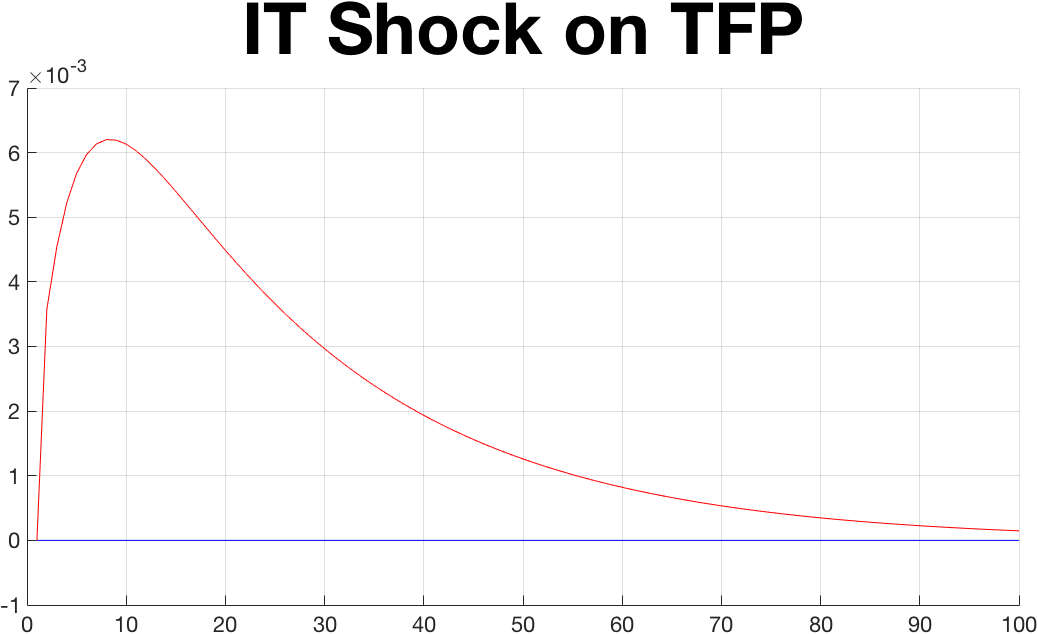
\includegraphics[scale = 0.13]{\ourFigPath Figures/fig_IT_Shock_on_TFP__}\\
\vspace{0.3cm}
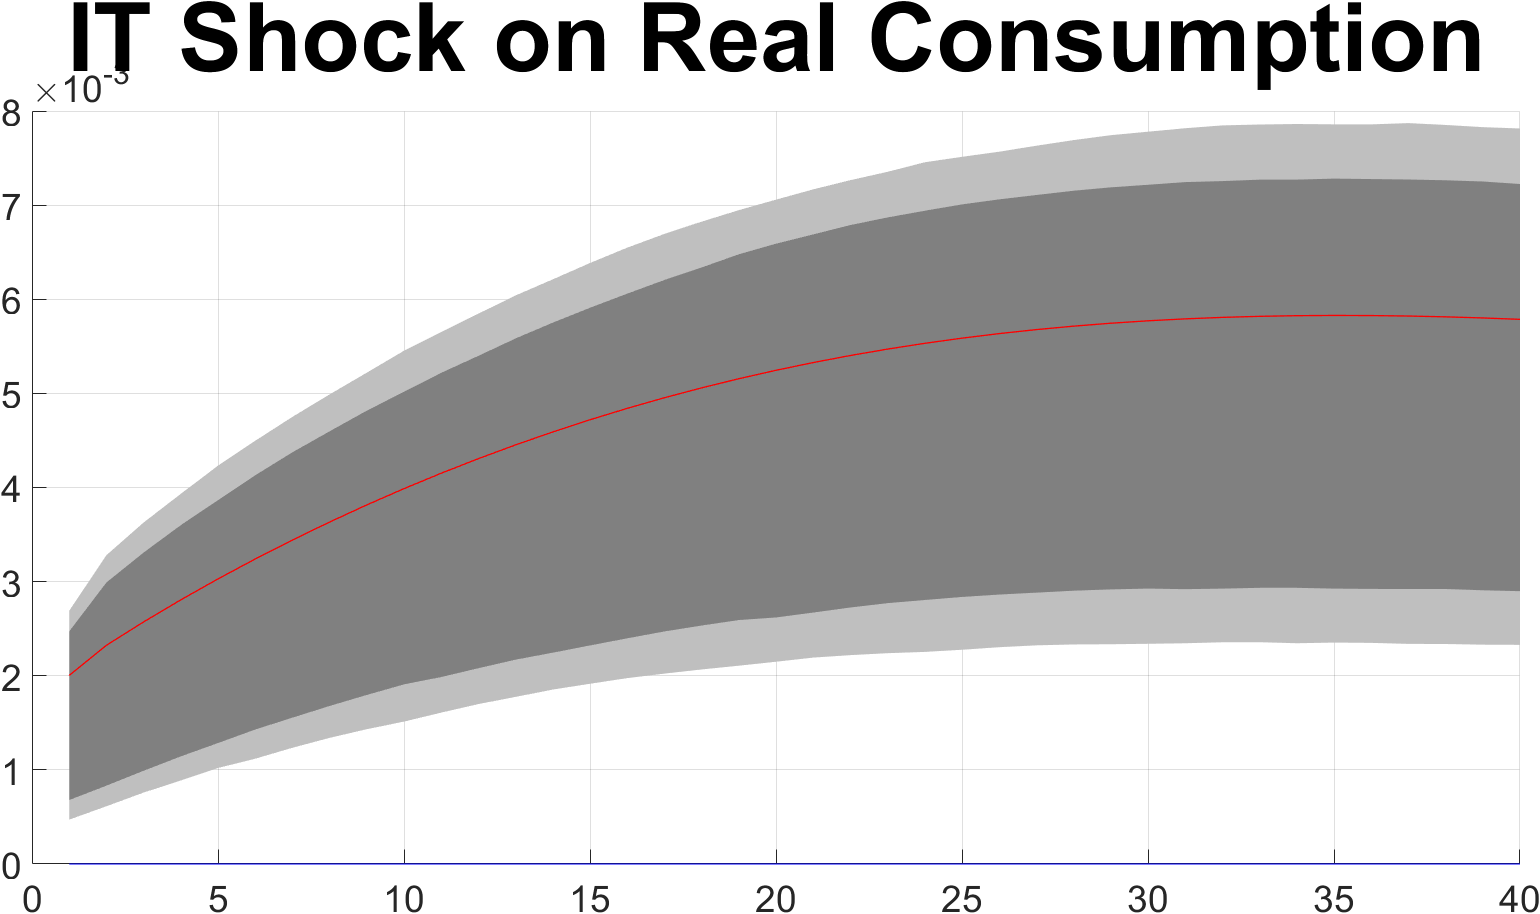
\includegraphics[scale = 0.13]{\ourFigPath Figures/fig_IT_Shock_on_Real_Consumption__}\\ 
\vspace{0.3cm}
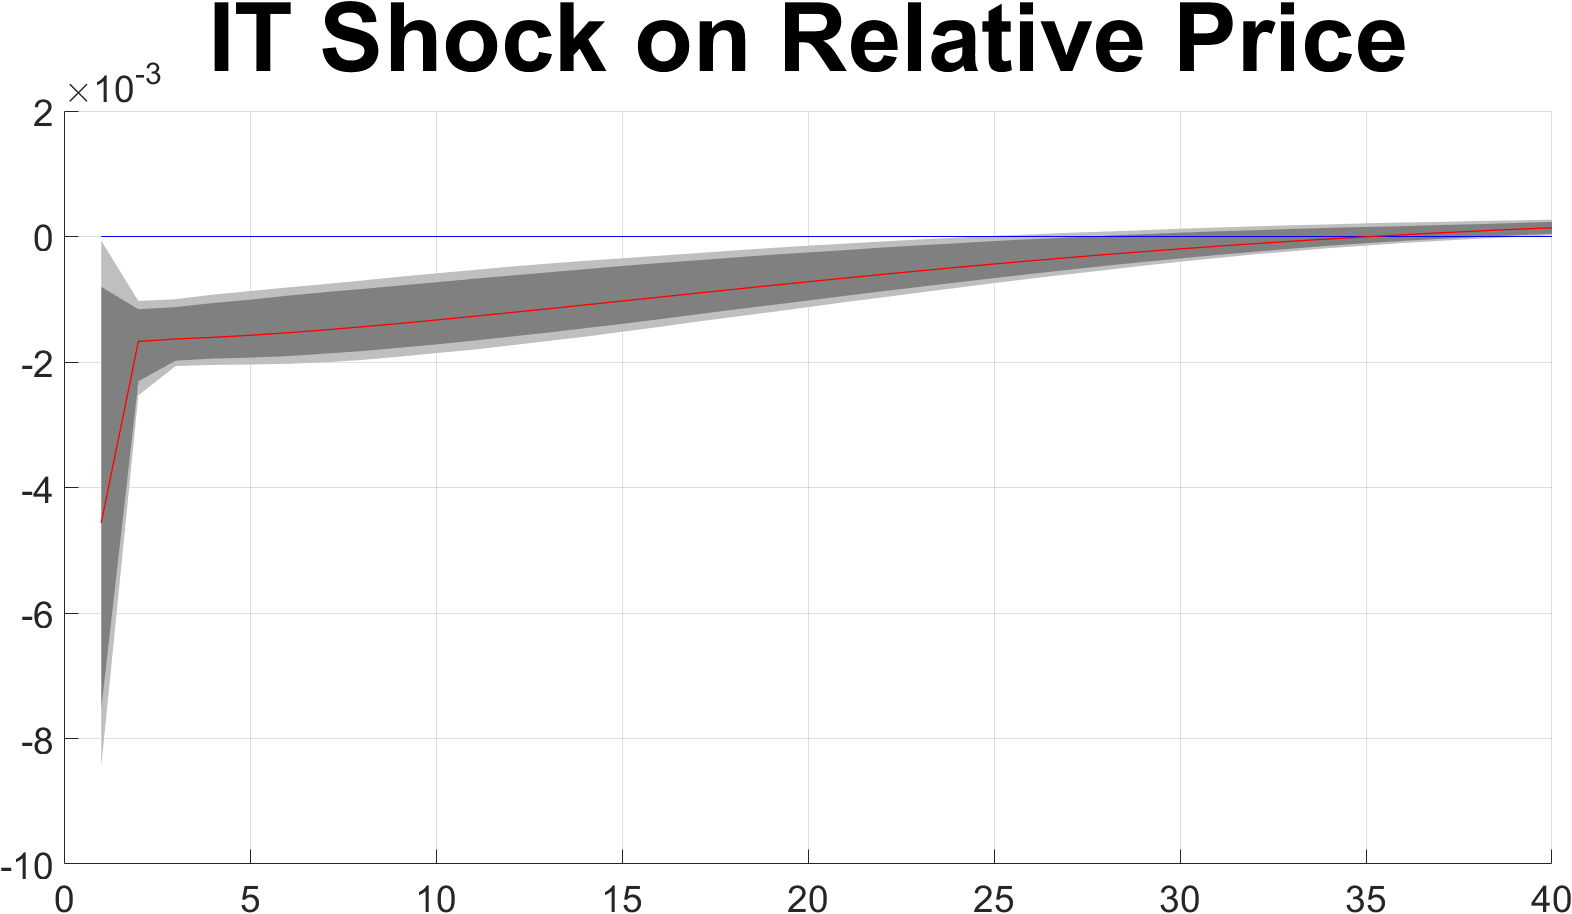
\includegraphics[scale = 0.13]{\ourFigPath Figures/fig_IT_Shock_on_Relative_Price__}\\ 

\end{multicols}
\end{figure}


\end{frame}
%%%%%%%%%%%%%%%%%%%%%%%%%%%%%


%%%%%%%%%%%%%%%%%%%%%%%%%
\begin{frame}
\frametitle{More VAR responses}

\vspace{-0.2cm}
\begin{figure}
\begin{multicols}{2}
\centering 
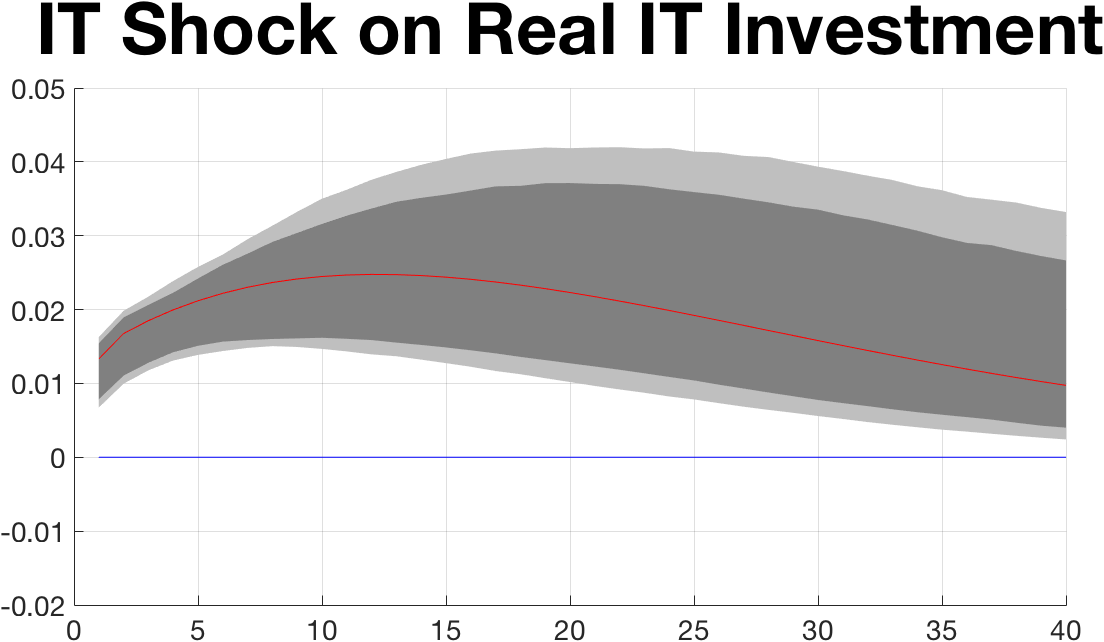
\includegraphics[scale = 0.13]{\ourFigPath Figures/fig_IT_Shock_on_Real_IT_Investment__}\\
\vspace{0.3cm}
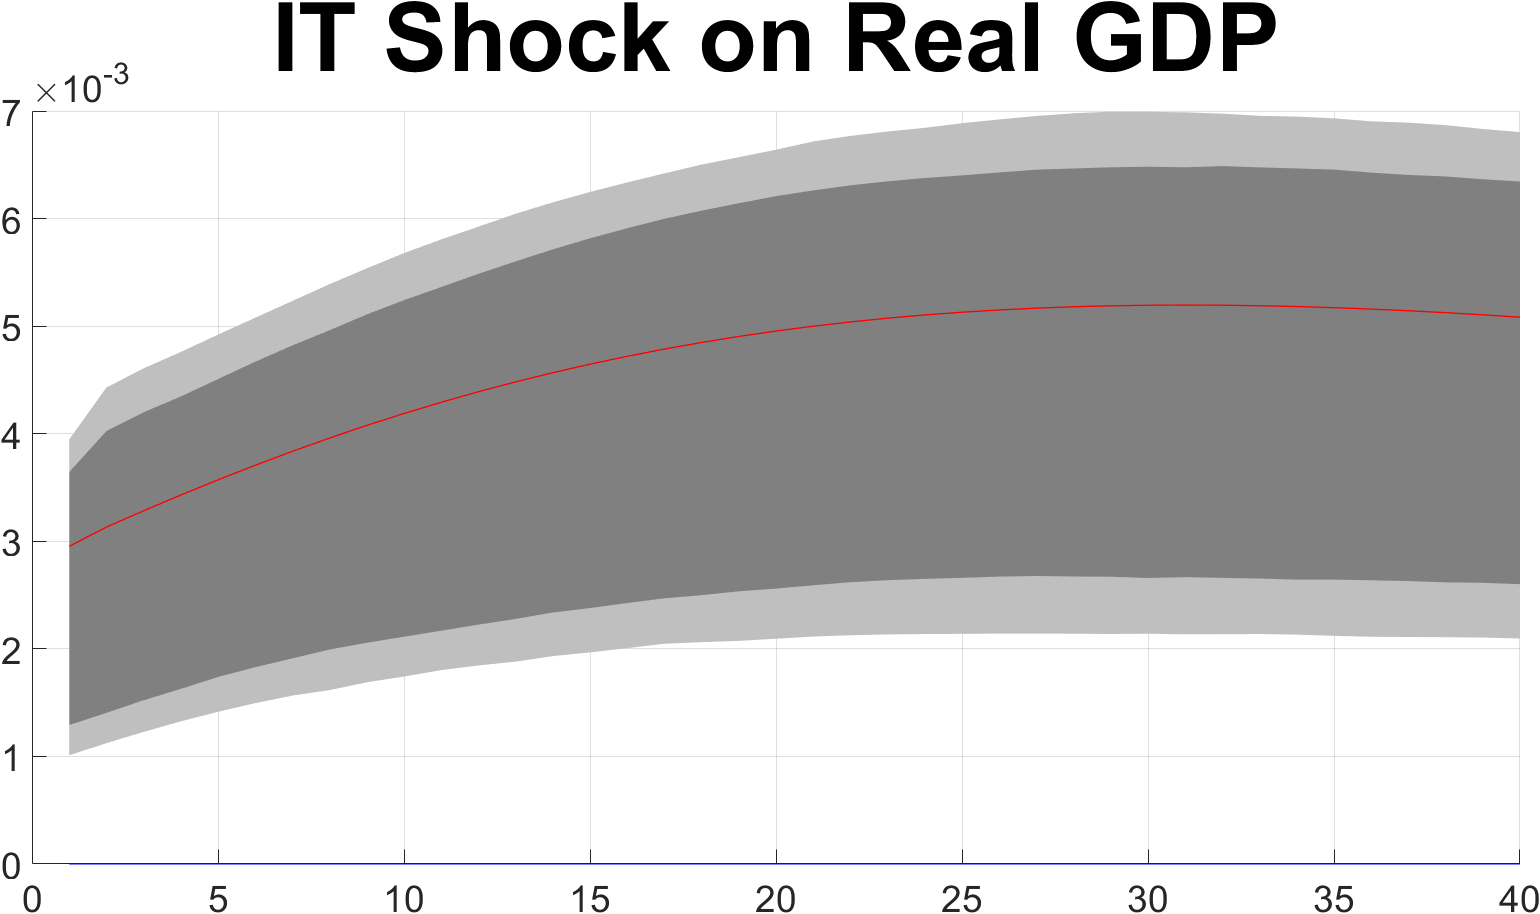
\includegraphics[scale = 0.13]{\ourFigPath Figures/fig_IT_Shock_on_Real_GDP__}\\ 
\vspace{0.3cm}
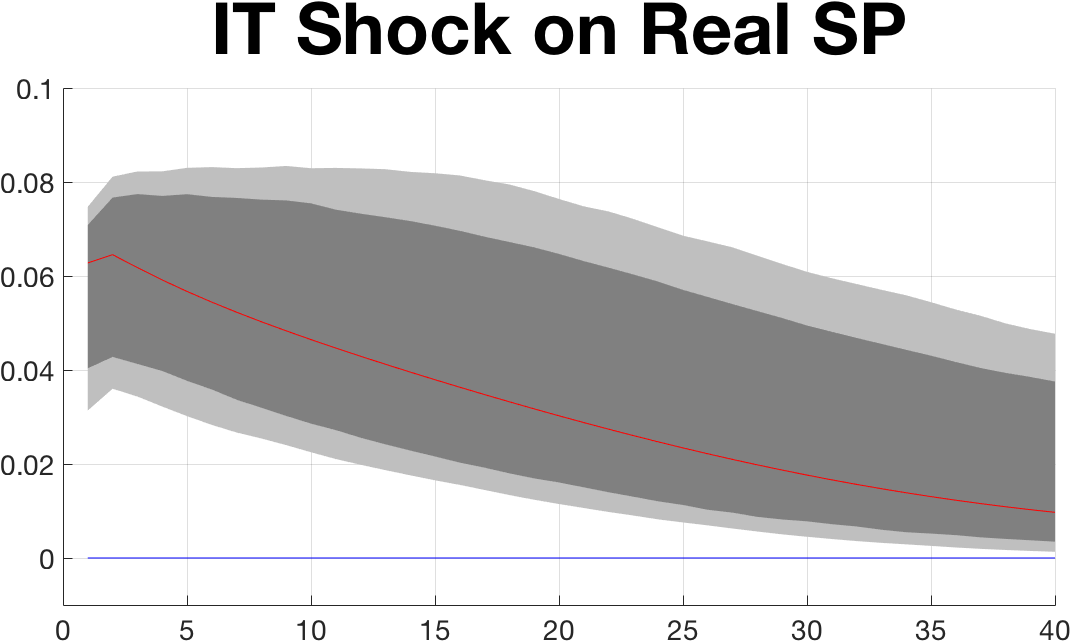
\includegraphics[scale = 0.13]{\ourFigPath Figures/fig_IT_Shock_on_Real_SP__}\\ 

\end{multicols}
\end{figure}


\end{frame}
%%%%%%%%%%%%%%%%%%%%%%%%%%%%%


%%%%%%% Slide %%%%%%
\begin{frame}
	\frametitle{3) Model}
	

\begin{equation}\label{eq:prodfuncfinal}
y_{c,t} = N_t  \  \ \Gamma_{c,t}  \  \ k_{i,t}^{\gamma} \ \  h_{1,t}^{1 - a- b} k_{c,1,t}^a k_{i,1,t}^b
\end{equation}

\


\begin{equation}\label{eq:prodfuncinter}
y_{i,t} = N_t \ \ \Gamma_{i,t} \ \ k_{i,t}^{\gamma} \ \  h_{2,t}^{1 - a- b} k_{c,2,t}^a k_{i,2,t}^b
\end{equation}

\

The uses of the outputs are
$$
y_{c,t} = c_t + i_{c,t} \ \ \text{and} \ \ y_{i,t} = i_{i,t}
$$


\

\begin{itemize}
%\item News shock is $\varepsilon$, $N_{t} = \rho_N N_{t-1} + \varepsilon_{t-k}$
\item Noise shock (contemporaneous) is $\eta$, $E_t \Gamma_{i,t} = \Gamma_{i,t} + \eta_t$
\end{itemize}

\end{frame}
%%%%%%%%%%%%%%%%%

%%%%%%%%%%%%%%%%%%%%%%%%%
\begin{frame}
\frametitle{Model responses}

\vspace{-0.2cm}
\begin{figure}
\begin{multicols}{2}
\centering 
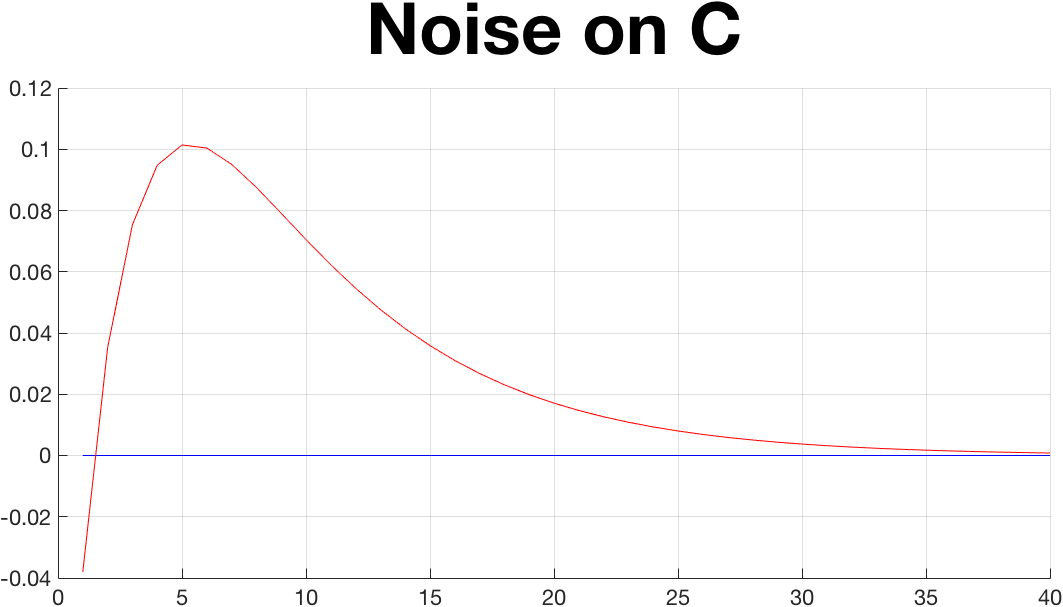
\includegraphics[scale = 0.13]{\ourFigPath Figures/fig_Noise_on_C__}\\
\vspace{0.3cm}
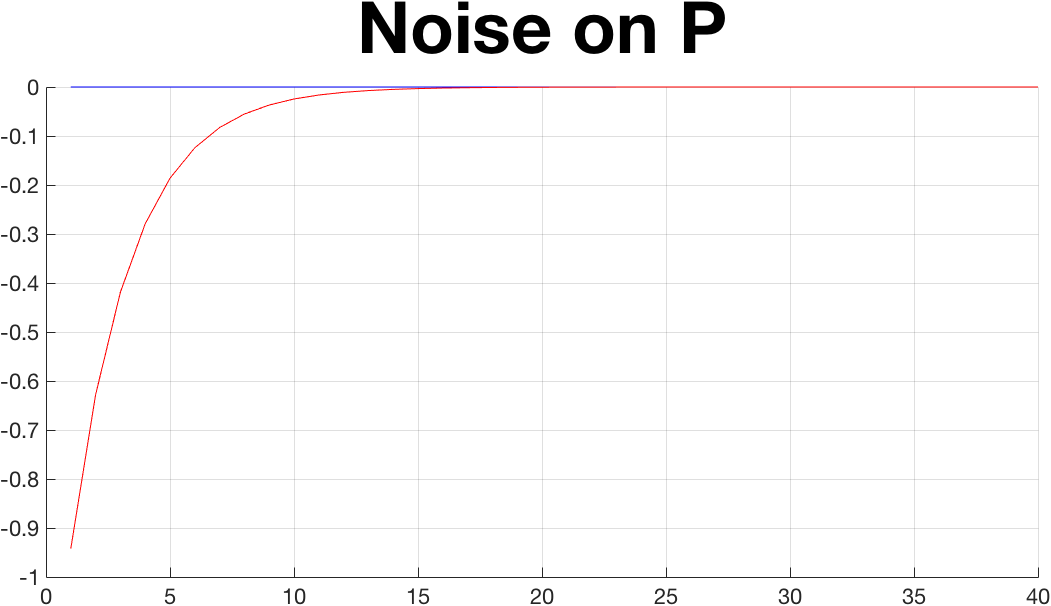
\includegraphics[scale = 0.13]{\ourFigPath Figures/fig_Noise_on_P__}\\ 
\vspace{0.3cm}
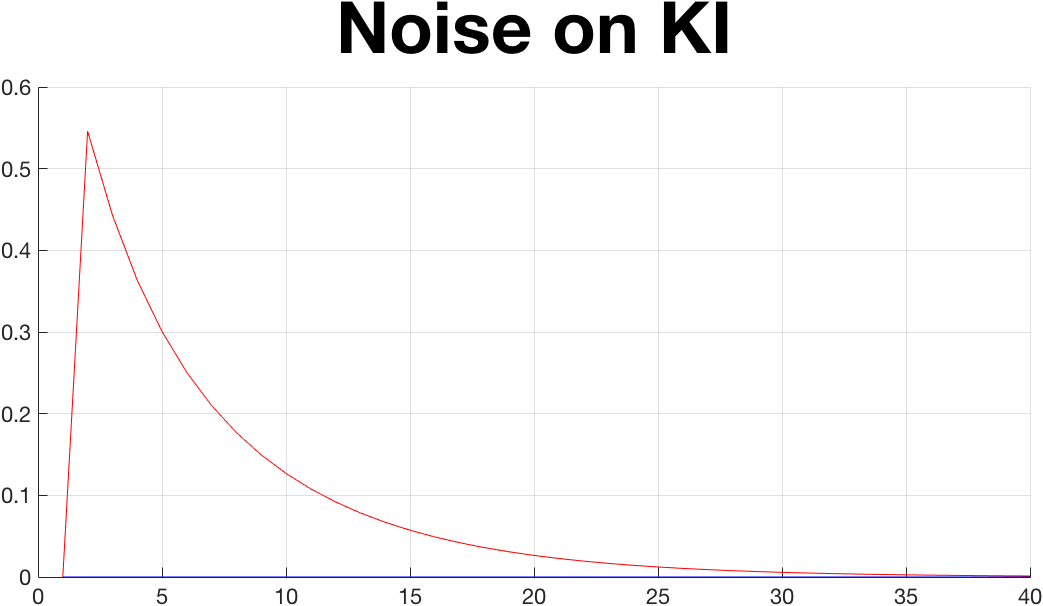
\includegraphics[scale = 0.13]{\ourFigPath Figures/fig_Noise_on_KI__}\\ 
\vspace{0.3cm}
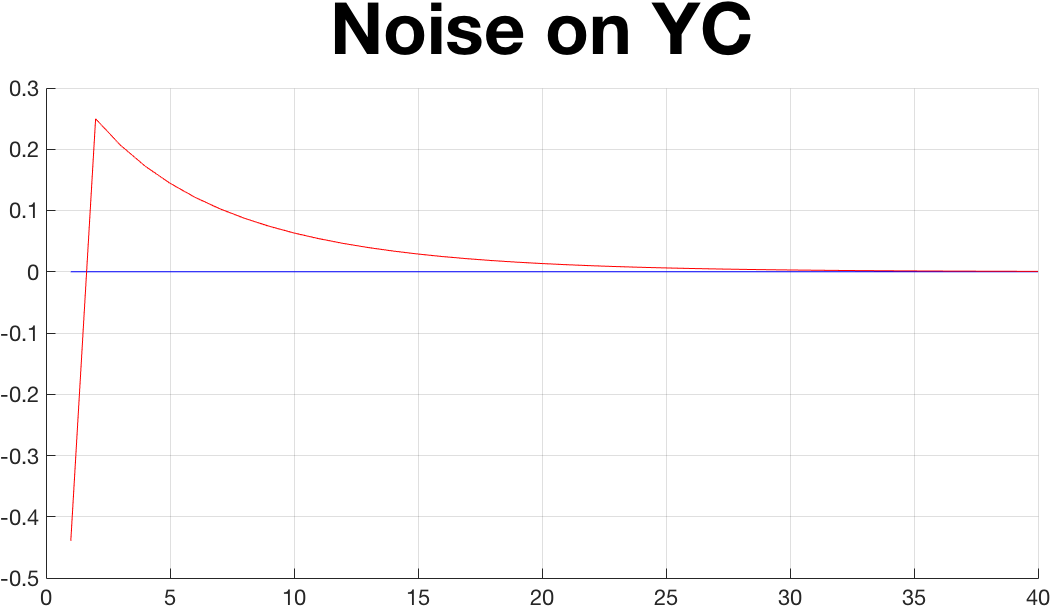
\includegraphics[scale = 0.13]{\ourFigPath Figures/fig_Noise_on_YC__}\\ 
\end{multicols}
\end{figure}


\end{frame}
%%%%%%%%%%%%%%%%%%%%%%%%%%%%%	


%%%%%%%        Slide    %%%%%%%%%%%%%%%%%%
\begin{frame}
\frametitle{Next steps}

\begin{itemize}
\item Estimate the spillover parameter $\gamma$ through IR-matching

\

\item Robustness checks / improving the VAR / completing the VECM

\

\item Your thoughts?
\end{itemize}


\end{frame}


%%%%%%%%%%%%%%%%%%%%%%%%%















\end{document}
